% 提案手法は分散グラフ上における RW エンジンである. そのため本章では関連研究について,「Random Walk エンジン」「単一データセンター内における分散グラフ処理システム」「地理的分散環境におけるグラフ処理システム」の 3 つに分けて整理する. その後, 本研究の位置づけを述べる. 

提案手法は分散グラフ上における RW エンジンに分類される. そのため本章では関連研究について,「Random Walk エンジン」「分散グラフ処理システム」の 2 つに分けて整理する. その後, 本研究の位置づけを述べる. 

\section{Random Walk エンジン}\label{sec:Random Walk エンジン}

Random Walk (RW) はグラフ解析において頻繁に用いられるため, その RW 演算を効率的に実行するシステムの開発は有意義なものであり, 複数の既存技術が存在する. 図 \ref{Random Walk エンジンの分類} にマシン数と目的による Random Walk エンジンの分類を示す. RW 実行エンジンはシングルマシンの手法, マルチマシンの手法の二つに分類することができる. さらにシングルマシンの手法の中には, メモリアクセスの改善を目的とした手法と大規模グラフでの実行を目的とした手法が存在する. 対してマルチマシンの手法の中には単一データセンター内での実行を目的とした手法があり, それに対する地理的分散環境下での実行を目的にしたのが提案手法である. 

% ThunderRW\cite{10.14778/3476249.3476257}, FlashMob\cite{10.1145/3477132.3483575} は共有メモリシステムにおける RW 演算の最適化を目的とした手法である. RW 演算ではランダムな隣接頂点への遷移を繰り返すため, 不規則なメモリアクセスが課題となる. そこで ThunderRW では異なる RW クエリの実行を切り替えることによりメモリアクセスの待ち時間を隠蔽した. また FlashMob では, Random Walker (RWer) は高次数頂点に高頻度で訪れることに注目し, 高次数頂点の隣接辺の事前サンプリングを行うことで, RWer の遷移を DRAM への Sequential Read に置き換え, メモリアクセスのオーバヘッドを削減した. 
ThunderRW\cite{10.14778/3476249.3476257}, FlashMob\cite{10.1145/3477132.3483575} はシングルマシンで動作するメモリアクセスの改善を目的とした手法である. RW 演算ではランダムな隣接頂点への遷移を繰り返すため, 不規則なメモリアクセスが課題となる. そこで ThunderRW では異なる RW クエリの実行を切り替えることによりメモリアクセスの待ち時間を隠蔽した. また FlashMob では, Random Walker (RWer) は高次数頂点に高頻度で訪れることに注目し, 高次数頂点の隣接辺の事前サンプリングを行うことで, RWer の遷移を DRAM への Sequential Read に置き換え, メモリアクセスのオーバヘッドを削減した. これらの手法は全体グラフが一つのマシンに格納されていることを前提としており, 分散マシンに拡張するのが困難である. そのため分散環境を想定する提案手法ではこれらの手法を導入することができない.  

% DrunkardMob\cite{10.1145/2507157.2507173}, GraphWalker\cite{254449}, NosWalker\cite{10.1145/3582016.3582025} はシングルマシンで動作する Out-of-Core RW エンジンである. Out-of-Core RW エンジンでは, 全てのグラフデータをメモリに載せて演算を行うのではなく, 必要なグラフデータを逐一メモリにロードしながら RW 演算を実行する. DRAM に対して低価格である SSD を利用してグラフデータを保持するため, 大規模グラフ上における RW 演算をより低コストで実行することが可能になる. NosWalker では, エッジサンプリングはエッジデータのみ, walker のアップデート処理は頂点データのみが必要となる RW の特性に注目し, それぞれの処理を分離する walker 指向の非連結アーキテクチャを採用している. 
DrunkardMob\cite{10.1145/2507157.2507173}, GraphWalker\cite{254449}, NosWalker\cite{10.1145/3582016.3582025} はシングルマシンで動作する大規模グラフでの実行を目的とした手法である. これらの手法は Out-of-Core RW エンジンといい, 全てのグラフデータをメモリに載せて演算を行うのではなく, 必要なグラフデータを逐一メモリにロードしながら RW 演算を実行する. DRAM に対して低価格である SSD を利用してグラフデータを保持するため, 大規模グラフ上における RW 演算をより低コストで実行することが可能になる. 最先端手法である NosWalker では, エッジサンプリングはエッジデータのみ, walker のアップデート処理は頂点データのみが必要となる RW の特性に注目し, それぞれの処理を分離する walker 指向の非連結アーキテクチャを採用している. これらの手法は, 大規模グラフでの RW 実行をシングルマシンで行うことによりコストを抑えようとしているため, 分散環境を許容している本研究とは目的と手段がそれぞれ異なる.

% KnightKing\cite{10.1145/3341301.3359634} はグラフデータを分散クラスタ上で保持する分散グラフ RW エンジンである. KnightKing には汎用性の高い API が設定されており, PPR, DeepWalk, MetaPath, Node2vec といった複数種類の RW を実行することができる. さらに KnightKing の貢献として, rejection ベースのエッジサンプリング手法による, 高次 RW アルゴリズムのコスト削減がある. RW 演算のボトルネックはエッジのサンプリング処理にあると言われており, walker の現在の状態, 前回訪れた頂点, 現在滞在している頂点のエッジの性質に依存するような動的サンプリングを必要とする高次 RW は顕著にその傾向を示している. KnightKing の rejection ベースのエッジサンプリングは O(d) (d: 頂点における次数)かかっていたエッジの動的サンプリングを O(1) (前計算 O(n), n: 頂点数) に削減した.
KnightKing\cite{10.1145/3341301.3359634} はマルチマシンで動作する単一データセンター内での実行を目的とした手法である. KnightKing には汎用性の高い API が設定されており, PPR, DeepWalk, MetaPath, Node2vec といった複数種類の RW を実行することができる. さらに KnightKing の貢献として, rejection ベースのエッジサンプリング手法による, 高次 RW アルゴリズムのコスト削減がある. RW 演算のボトルネックはエッジのサンプリング処理にあると言われており, walker の現在の状態, 前回訪れた頂点, 現在滞在している頂点のエッジの性質に依存するような動的サンプリングを必要とする高次 RW は顕著にその傾向を示している. KnightKing の rejection ベースのエッジサンプリングは O(d) (d: 頂点における次数)かかっていたエッジの動的サンプリングを O(1) (前計算 O(n), n: 頂点数) に削減した. 提案手法の実験における RW はエッジの静的サンプリングのみを対象としているため, KnightKing のrejection ベースのエッジサンプリングは使用していない. しかし, 提案手法においてエッジの動的サンプリングを導入する場合は, この rejection サンプリングを利用することになる. また, KnightKing は単一データセンター内での実行を目的としているため, TCP 通信を使った同期処理を採用しているが, 本研究が想定する地理的分散環境下では性能が劣化する. 

本研究が想定しているのはマルチマシンかつ地理的に分散した環境である. そのため, シングルマシンでの動作を前提とした手法や単一データセンター内での動作を前提とした手法は想定環境に合致せず, 本来のパフォーマンスを発揮することができない. 

\begin{figure}[t]
    \centering
    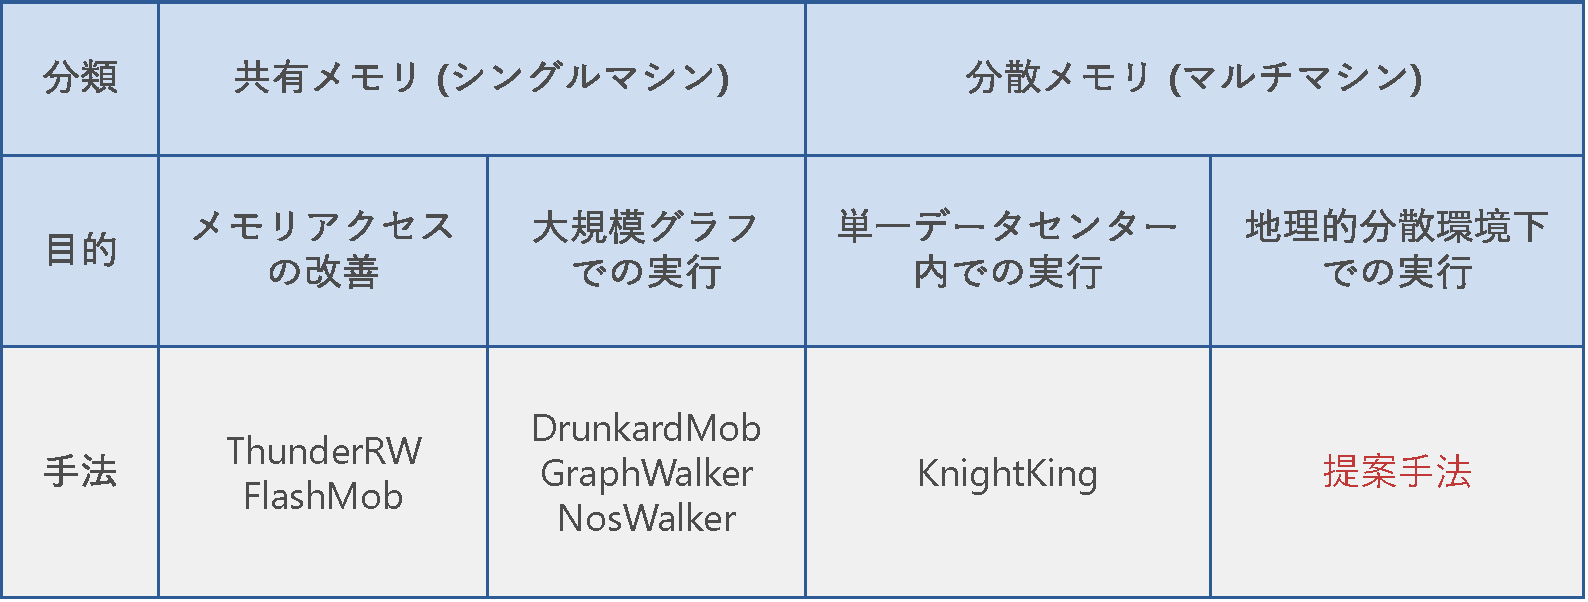
\includegraphics[scale=0.5]{figure/RWEngine.pdf}
    \caption{Random Walk エンジンの分類.}
    \label{Random Walk エンジンの分類}
\end{figure}

\section{分散グラフ処理システム}\label{sec:分散グラフ処理システム}

近年のグラフデータの増加に伴い, 分散クラスタ上で動作する分散グラフ処理システムの重要性が高まっている. 図 \ref{分散グラフ処理システムの分類} に分散グラフ処理システムの分類を示す. まず, 分散グラフ処理システムは単一データセンター内での実行を目的とした手法と地理的分散環境下での実行を目的とした手法に分けられる. また, プログラミングモデルという観点で, vertex-centric な手法と walker-centric な手法に分けられる. 提案手法は, 地理的分散環境下での実行を目的とした walker-cenric な手法である. 

% 近年のグラフデータの増加に伴い, 分散クラスタ上で動作する分散グラフ処理システムの重要性が高まっている. 分散グラフ処理における主流なプログラミングモデルとして, Bulk Synchronous Parallel (BSP) モデルがある. BSP モデルは, スーパーステップと呼ばれる単位で処理を繰り返し行うモデルであり, このスーパーステップは主に
% \begin{itemize}
%     \item サーバごとでの計算
%     \item サーバ間同期
% \end{itemize}
% で構成される. 同期型である BSP モデルを非同期型にすることで処理を高速化する手法も存在する\cite{BAP}\cite{AAP}\cite{Gluon-Async}が, 実装の複雑化や, データセンター内等の高帯域環境では同期のオーバヘッドがさほど大きくならないことから, BSP モデルが採用されることが多い. 

まず単一データセンター内での処理を目的とした手法について述べる. ここで使われる分散グラフ処理における主流なプログラミングモデルとして, Bulk Synchronous Parallel (BSP) モデルがある. BSP モデルは, スーパーステップと呼ばれる単位で処理を繰り返し行うモデルであり, このスーパーステップは主に
\begin{itemize}
    \item サーバごとでの計算
    \item サーバ間同期
\end{itemize}
で構成される. BSP モデルの分散グラフシステムのうち, 頂点の状態に注目した手法\cite{Pregel}\cite{10.1145/2741948.2741970}\cite{10.5555/2387880.2387883}\cite{10.5555/3026877.3026901}\cite{Gluon}は vertex-centric なモデルと呼ばれる. vertex-centric モデルにおける各スーパーステップでは, 各頂点が, 直前のスーパーステップで送られたメッセージに基づいて自身の状態を更新し, 結果を他の頂点に送信する. ユーザは頂点における更新に関する処理を記述するのみであり, PageRank, Single Source Shortest Path, connected components 等の多くのグラフアルゴリズムはこの vertex-centric の形で書き下すことが可能である. 対して\ref{sec:Random Walk エンジン} 節で紹介した KnightKing は, 処理単位が RWer であることから walker-centric モデルと呼ばれている. 図\ref{walker centric モデル (同期型) の概要} は walker-centric モデルの概要を示しており, 各スーパーステップでは, 
\begin{itemize}
    \item 各 RWer がユーザー定義の RW を実行 (1 ステップ進める) し, 状態を更新
    \item 状態を更新した RWer の内, 他のサーバが管理する頂点へ遷移した RWer を送信し, 全サーバで同期
\end{itemize}
を行う. vertex-centric モデルを採用しないのは, RW における RWer の概念は, 既存の vertex-centric モデルのシステムではメッセージとして扱われるため, RWer の状態更新の追跡や最適化のための機能が失われる可能性が高いためである. vertex-centric モデルの手法においては, BSP モデルのような同期処理によって全体としての計算を進めていく手法の他に, 非同期処理を採用する手法も存在する \cite{BAP}\cite{AAP}\cite{Gluon-Async} .  非同期処理では, BSP モデルのように各サーバでの演算が終わった後の同期を行わない. これにより高速な Worker は他の Worker を待つことなく実行を継続でき, 同期処理での問題となる stragglers (遅い Worker) の発生による待ち時間の増加を防ぐことができる. しかし, BSP モデルに対し実装が複雑になることや, 実行するグラフアルゴリズムによっては冗長な反復計算が増えるといった問題点がある. また, データセンター内等の高帯域環境では同期のオーバヘッドがさほど大きくならないことから, 非同期処理を導入したことによる高速化の効果はさほど高くない. 

\begin{figure}[t]
    \centering
    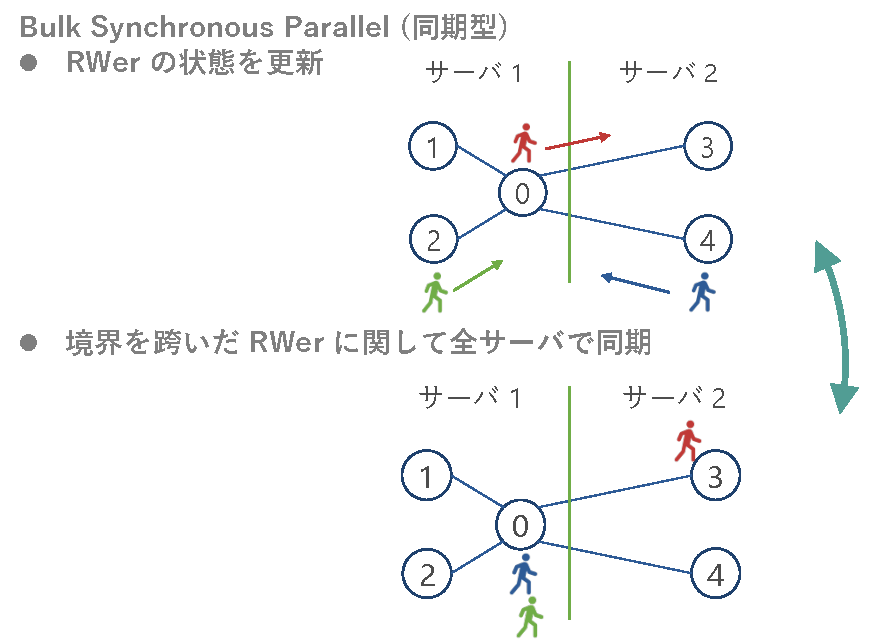
\includegraphics[scale=0.7]{figure/walkercentric.pdf}
    \caption{walker centric モデル (同期型) の概要.}
    \label{walker centric モデル (同期型) の概要}
\end{figure}



% 地理的に分散した環境でグラフデータが生成, 管理される状態を想定したグラフ解析システム\cite{10.5555/3277180.3277185}\cite{8486361}\cite{10.1145/3397271.3401157}も存在する. 
% グラフクエリは, PageRank Web 検索\cite{334}, SNS 検索\cite{10.5555/2535461.2535468}, ナレッジグラフ検索\cite{10.1145/3331184.3331252}など, 多くの一般的なインターネットサービスの基盤となっているが, このようなグラフクエリで処理されるグラフは巨大であり, 変化の速度も速い\cite{10.1145/2723372.2735365}ため, 広域ネットワーク (WAN) でのデータ転送のコストが高い. さらに GDPR 等のプライバシー規制も相まって, グラフデータ全体を一箇所に集めることは極めて困難である. そのため, 地理的に分散した環境下における効率的なグラフ処理システムの開発が重要となる. 

次に地理的分散環境下での処理を目的とした手法について述べる. 前段落で紹介した分散グラフ処理システムは, 単一のデータセンター内のサーバクラスタのような高帯域・低遅延な環境下で実行することを想定しているため, 低帯域・高遅延の WAN での実行では大きく性能が劣化する. これは BSP モデルのスーパーステップにおける隣接ノード間の通信がアルゴリズムの収束まで何度も繰り返されるからである. そこで, 既存の地理的分散環境下を想定した分散グラフ処理システム\cite{8486361}\cite{10.1145/3397271.3401157} は前段落における一般的な vertex-centric モデルの通信削減に注力している. HSP モデル\cite{8486361} では, サーバ間の同期をデータセンター内とデータセンター間で 2 階層に分けることにより, データセンター間での通信量を削減する. また, GeoGraph\cite{10.1145/3397271.3401157} では, WAN レイテンシに基づきデータセンターをグループ化し, そのグループ間の通信量を削減する. しかし, これらの手法は提案手法のように RW 実行を目的とした場合, 利点がなくなる. なぜなら, vertex-centric モデルの計算では, 頂点間の同期の順番を入れ替えることで, 値の収束を早めたりサーバ間の通信量を減らすことができるが, walker-centric モデルでは RWer の遷移先を変更できないためサーバ間の通信量を減らすことができないためである. つまり HSP モデル, GeoGraph を walker-centric モデルに 適用させることはできない. 

\begin{figure}[t]
    \centering
    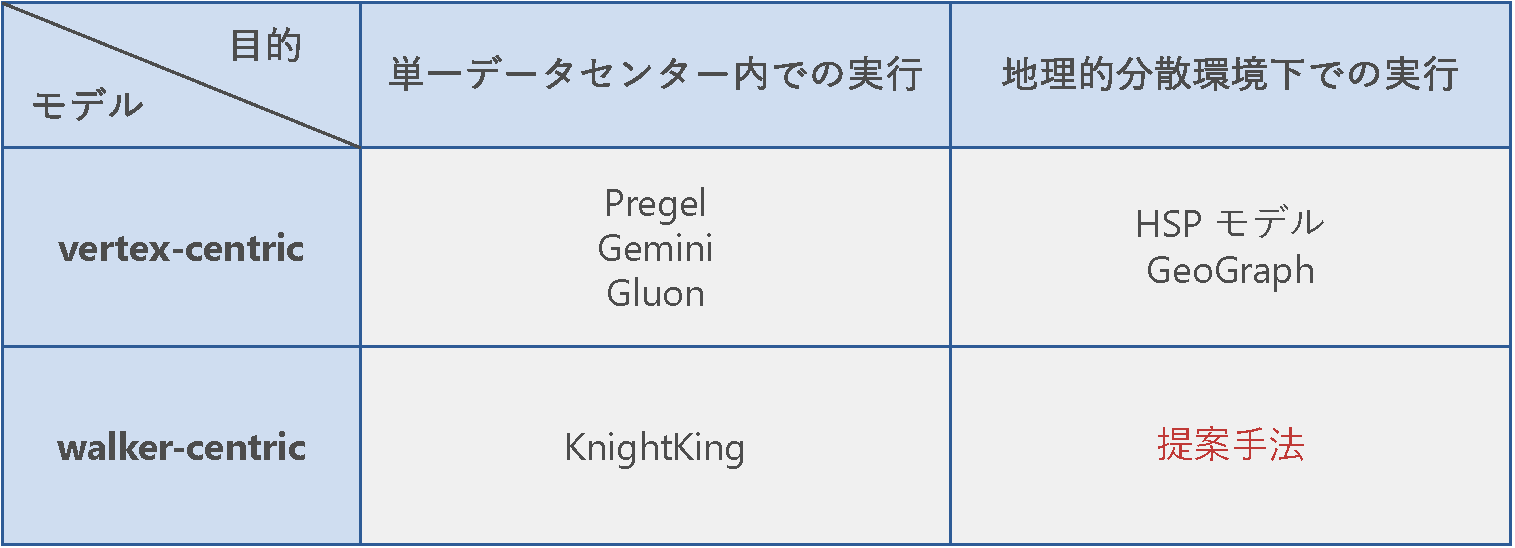
\includegraphics[scale=0.5]{figure/DistributedSystem.pdf}
    \caption{分散グラフ処理システムの分類.}
    \label{分散グラフ処理システムの分類}
\end{figure}

\section{本研究の位置づけ}

% まず, Random Walk エンジンとしての本研究の位置づけについて述べる. 図 \ref{Random Walk エンジンの分類} にマシン数と目的による Random Walk エンジンの分類を示す. 提案手法は, マルチマシンによる地理的分散環境下での実行を目的とした手法に分類される. ThunderRW, FlashMob 等のシングルマシンにおけるメモリアクセスの改善を目的とした手法は, 分散マシンに拡張するのが困難であり, さらにグラフの変化に対応することができないため, 本研究が想定する地理的分散環境下への適用が困難である. DrunkardMob, GraphWalker, NosWalker は大規模グラフでの RW 実行をシングルマシンで行うことによりコストを抑えようとしているため, 分散環境を許容している本研究とは目的と手段がそれぞれ異なる. KnightKing は単一データセンターでの RW 実行を目的とした, 分散グラフ RW エンジンであり, TCP 通信による同期処理を採用している. しかし本研究が想定する地理的分散環境下では RTT・パケットロス率が高くなり, TCP 通信のスループットが大幅に低下するため, 同期のオーバヘッドが大きくなる. また, RW の特徴である終盤の少数の RWer のためにわざわざ同期処理を行うのは無駄が多い. 

% 次に分散グラフ処理システムとしての本研究の位置づけについて述べる. 図 \ref{分散グラフ処理システムの分類} に分散グラフ処理システムの分類を示す. 提案手法は, 地理的分散環境下における walker-centric モデルの手法に分類される. HSP モデル, GeoGraph は vertex-centric モデルにおける通信削減を目的としている. vertex-centric モデルの計算では, 頂点間の同期の順番を入れ替えることで, 値の収束を早めたりサーバ間の通信量を減らすことができるが, walker-centric モデルでは RWer の遷移先を変更できないためサーバ間の通信量を減らすことができない. つまり HSP モデル, GeoGraph を walker-centric モデルに 適用させることはできない. 

提案手法は既存の RW エンジンとは異なり, 地理的分散環境下における実行に対応することを目的としている. また, 既存の分散グラフ処理システムとは異なり, 地理的分散環境下への対応かつ RW 実行への対応を目的とする. 目的達成のため, 提案手法では UDP 通信を使った非同期処理を採用した. UDP 通信を使用することで地理的分散環境下における低帯域・高遅延な通信環境であっても影響が少なく, システムのスケーラビリティ向上に貢献する. そして非同期処理を採用することにより地理的分散環境下での RW 実行の同期のオーバヘッドが解消され, データセンターごとの自律的な RW 実行に対応することができるようになった. また, 提案手法は終了後の RWer の経路情報を再利用することにより RW 遷移による通信を削減することができる. 